%\documentclass[12pt,twoside]{article}
\documentclass[conference]{IEEEtran}  % this should work with your LaTeX installation; else download extra package (www.ctan.org/pkg/ieeetran) or remove IEEE usage below

%%%%%%% Fill this out:
\newcommand{\trtitle}{Detecting Opinion Spammer Groups}
\newcommand{\titleshort}{NNs for Artificial Agents} % title for header:
\newcommand{\authorlastnames}{Adams, Jefferson, Washington} % alphabetical for seminars
\newcommand{\trcourse}{Knowledge Processing in Intelligent Systems: Practical Seminar}
\newcommand{\trgroup}{Knowledge Technology, WTM}
\newcommand{\truniversity}{Department of Informatics, University of Hamburg}
%%%%%%%%%%%%%%%%%%%%%%%%%%%%%%%%%%%%%%%%%%%%%%%%%%%%%%%%%%%%%
% Languages:

% If the thesis is written in English:
\usepackage[english]{babel} 						
\selectlanguage{english}

%%%%%%%%%%%%%%%%%%%%%%%%%%%%%%%%%%%%%%%%%%%%%%%%%%%%%%%%%%%%%
% Bind packages:
\usepackage{lipsum}

\usepackage{acronym}                    % Acronyms
\usepackage{algorithmic}								% Algorithms and Pseudocode
\usepackage{algorithm}									% Algorithms and Pseudocode
\usepackage{amsfonts}                   % AMS Math Packet (Fonts)
\usepackage{amsmath}                    % AMS Math Packet
\usepackage{amssymb}                    % Additional mathematical symbols
\usepackage{amsthm}
\usepackage{booktabs}                   % Nicer tables
%\usepackage[font=small,labelfont=bf]{caption} % Numbered captions for figures
\usepackage{color}                      % Enables defining of colors via \definecolor
\definecolor{uhhRed}{RGB}{254,0,0}		  % Official Uni Hamburg Red
\definecolor{uhhGrey}{RGB}{122,122,120} % Official Uni Hamburg Grey
\usepackage{fancybox}                   % Gleichungen einrahmen
\usepackage{fancyhdr}										% Packet for nicer headers
%\usepackage{fancyheadings}             % Nicer numbering of headlines

%\usepackage[outer=3.35cm]{geometry} 	  % Type area (size, margins...) !!!Release version
%\usepackage[outer=2.5cm]{geometry} 		% Type area (size, margins...) !!!Print version
%\usepackage{geometry} 									% Type area (size, margins...) !!!Proofread version
\usepackage{geometry} 	  % Type area (size, margins...) !!!Draft version
\geometry{a4paper,body={7.0in,9.1in}}

\usepackage{graphicx}                   % Inclusion of graphics
%\usepackage{latexsym}                  % Special symbols
\usepackage{longtable}									% Allow tables over several parges
\usepackage{listings}                   % Nicer source code listings
\usepackage{multicol}										% Content of a table over several columns
\usepackage{multirow}										% Content of a table over several rows
\usepackage{rotating}										% Alows to rotate text and objects
%\usepackage[hang]{subfigure}            % Allows to use multiple (partial) figures in a fig
%\usepackage[font=footnotesize,labelfont=rm]{subfig}	% Pictures in a floating environment
\usepackage{tabularx}										% Tables with fixed width but variable rows
\usepackage{url,xspace,boxedminipage}   % Accurate display of URLs

%%%%%%%%%%%%%%%%%%%%%%%%%%%%%%%%%%%%%%%%%%%%%%%%%%%%%%%%%%%%%
%Own packages
\usepackage{graphicx}
\usepackage{subfig}
\usepackage[T1]{fontenc}

%%%%%%%%%%%%%%%%%%%%%%%%%%%%%%%%%%%%%%%%%%%%%%%%%%%%%%%%%%%%%
% Configurationen:

\hyphenation{whe-ther} 									% Manually use: "\-" in a word: Staats\-ver\-trag

%\lstloadlanguages{C}                   % Set the default language for listings
\DeclareGraphicsExtensions{.pdf,.svg,.jpg,.png,.eps} % first try pdf, then eps, png and jpg
\graphicspath{{./src/}} 								% Path to a folder where all pictures are located
\pagestyle{fancy} 											% Use nicer header and footer

% Redefine the environments for floating objects:
\setcounter{topnumber}{3}
\setcounter{bottomnumber}{2}
\setcounter{totalnumber}{4}
\renewcommand{\topfraction}{0.9} 			  %Standard: 0.7
\renewcommand{\bottomfraction}{0.5}		  %Standard: 0.3
\renewcommand{\textfraction}{0.1}		  	%Standard: 0.2
\renewcommand{\floatpagefraction}{0.8} 	%Standard: 0.5

% Tables with a nicer padding:
\renewcommand{\arraystretch}{1.2}

%%%%%%%%%%%%%%%%%%%%%%%%%%%%
% Additional 'theorem' and 'definition' blocks:
\theoremstyle{plain}
\newtheorem{theorem}{Theorem}[section]
%\newtheorem{theorem}{Satz}[section]		% Wenn in Deutsch geschrieben wird.
\newtheorem{axiom}{Axiom}[section] 	
%\newtheorem{axiom}{Fakt}[chapter]			% Wenn in Deutsch geschrieben wird.
%Usage:%\begin{axiom}[optional description]%Main part%\end{fakt}

\theoremstyle{definition}
\newtheorem{definition}{Definition}[section]

%Additional types of axioms:
\newtheorem{lemma}[axiom]{Lemma}
\newtheorem{observation}[axiom]{Observation}

%Additional types of definitions:
\theoremstyle{remark}
%\newtheorem{remark}[definition]{Bemerkung} % Wenn in Deutsch geschrieben wird.
\newtheorem{remark}[definition]{Remark} 

%%%%%%%%%%%%%%%%%%%%%%%%%%%%
% Provides TODOs within the margin:
\newcommand{\TODO}[1]{\marginpar{\emph{\small{{\bf TODO: } #1}}}}

%%%%%%%%%%%%%%%%%%%%%%%%%%%%
% Abbreviations and mathematical symbols
\newcommand{\modd}{\text{ mod }}
\newcommand{\RS}{\mathbb{R}}
\newcommand{\NS}{\mathbb{N}}
\newcommand{\ZS}{\mathbb{Z}}
\newcommand{\dnormal}{\mathit{N}}
\newcommand{\duniform}{\mathit{U}}

\newcommand{\erdos}{Erd\H{o}s}
\newcommand{\renyi}{-R\'{e}nyi}
\usepackage{graphicx}

% correct bad hyphenation here
\hyphenation{}

%%%%%%%%%%%%%%%%%%%%%%%%%%%%%%%%%%%%%%%%%%%%%%%%%%%%%%%%%%%%%
% Document:
\begin{document}

\title{\trtitle}
\renewcommand{\headheight}{14.5pt}

%\fancyhead{}
%\fancyhead[LE]{  }
\fancyhead[LO]{\slshape \authorlastnames}
%\fancyhead[RE]{}
\fancyhead[RO]{ \slshape \titleshort}

% author names and affiliations
% use a multiple column layout for up to three different
% affiliations
\author{
\IEEEauthorblockN{Lars Stelzer}
\IEEEauthorblockA{lars.stelzer@studium.uni-hamburg.de}
\IEEEauthorblockA{7346178}
\and
\IEEEauthorblockN{Niklas von Boguszewski}
\IEEEauthorblockA{nvboguszewski@googlemail.com}
\IEEEauthorblockA{6790872}
\and
\begin{tabular}{lr}% 
	\trcourse\\ 
	\trgroup,
	\truniversity
\end{tabular}

}


       


% make the title area
\maketitle

\begin{abstract}
This paper aims to detect opinion spammer groups on the Yelp dataset.

Methode nennen

results zeigen (conclusion)

\end{abstract}

\IEEEpeerreviewmaketitle

\section{Introduction}
\label{sec:introduction}

Consumers' decisions are significantly influenced by product reviews. Due to the ongoing digitalization more and more consumers rely their decision making on online reviews. Online product reviews have by now become the second must trusted source of product information, followed by recommendations from family and friends. This happens due to the belief that online product reviews reflect recommendations of "real" people. %\cite {zhu2010marketing}
A rising online marketing budget has led to a larger influence and importance of online reviews in purchase and decision making. By the fact that positive/negative reviews are able to enhance/defame products organised opinion spamming started to take place. %\cite{kc2016dynamics}
Nowadays it is estimated that up to 20\% of online reviews could be fake. %\cite{wang2010statistic} 

These fake reviews are not the work of alone acting individuals, but more of organised payed group spammers \cite{choo2015detecting}. More often the media reports of such groups. For example in 2013 nineteen companies got fined for their practice of writing fake online reviews. These companies systematically paid freelance writers from Philippines, Bangladesh and Eastern Europe between \$1 to \$10 per review. (https://www.marketwatch.com/story/20-of-yelp-reviews-are-fake-2013-09-24)
With the growing popularity of these platforms and the direct influence on the businesses success the practice of leaving fake reviews for its own or the competitors’ business is becoming more common.Luca, M., and Zervas, G. (2016). Fake It Till You Make It: Reputation, Competition, and Yelp Review Fraud. Management Science, 62(12), 3412–3427. doi:10.1287/mnsc.2015.2304 
The \textit{New York Times} reported in 2011 on the case of businesses hiring workers to post fake 5-star Yelp reviews on their behalfs for as little as 25 cent per review. https://www.nytimes.com/2011/05/22/your-money/22haggler.html
In another case Samsung got a heavy penalty for paying people to post messages online that attacked HTC, their competitor, products while praising Samsung’s. https://abcnews.go.com/Technology/samsung-fined-paying-people-criticize-htcs-products/story?id=20671547

Yelp filters roughly 16 \% of its business reviews on its own. /cite Luca, M., and Zervas, G. (2016). Fake It Till You Make It: Reputation, Competition, and Yelp Review Fraud. Management Science, 62(12), 3412–3427. doi:10.1287/mnsc.2015.2304 
Still reportedly Yelp’s spokesman says 20-25 \% of the submitted reviews are “suspicious”. https://www.marketwatch.com/story/20-of-yelp-reviews-are-fake-2013-09-24

In Fig. 1 examples of spam reviews we researched are shown. These reviews were posted by the same person but for two different businesses. 

In this paper we propose a method to determine suspicious spammer groups accomplished by three steps. All these steps are based on the freely accessible Yelp.com dataset. Here we summarize the contributions of this paper as follows:
\begin{description}
\item[1.]
Firstly we create user groups based on the review time of the written review and the rating score given by the user. With this step we are able to create groups that reviewed the same business at nearly the same time giving the same rating score. Goal is to find groups that potentially work together writing fake reviews. 
\item[2.]
Followed by the creation of groups we determine features that help us to determine suspicious behaviour. In this paper we use three features that give hints if a user or group acts suspicious. We are looking at behavioral data like review time, rating score and textual similarity between reviews. 
\item[3.]
Based on our groups and features we are giving each group a score that determines how likely this group is an actual spammer group, called suspicious score. The suspicious score is calculated out of the key indicators given by the individual feature assigned to each group. 
\end{description}
The paper is structured as follows. Section II introduces related work in the field of spam detection. Section III gives more detailed information about the used Yelp.com dataset, platform and review system. Section IV describes our determined features. Section V our model which aims to find opinion spamming groups gets described. Section VI reports the experimental results. Finally, Section VII concludes and discusses the paper.


\section{Related Work}
\label{sec:related_work}

Over the last years the field of spam review detection has been experienced plenty of attention. The existing researches can be divided based on the data and features they analyze. Below are presented three different approaches to filter and detect spam. %\cite {xu2019cpm} 

\begin{description}
\item[1.]
\textit{Review spam detection:} this approach is based on the data of the review (e.g., textual content, meta data, etc.) to detect and filter spam reviews. %\cite {cardoso2018review, harris2012deceptive, ott-etal-2011-finding} 
\item[2.]  
\textit{Review spammer detection:} this approach is aiming to find the spammer it self. This can be, for example, achieved by identifying atypical behavior, such as posting time or geolocation. %\cite {mukherjee2013spotting, fei2013spammer, li2015pattern}
\item[3.]
\textit{Group spammer detection:} goal with this approach is to identify whole group of spammers due to the fact that group spammer are more influential and harmful than individual spammer.  %\cite {choo2015detecting, mukherjee2012groups, xu2019cpm}

\end{description}

Was haben andere gemacht

single fake review erkenne (3)

gruppen fake reviews erkennen

ergebnisse ...

gruppenansatz von paper CPM XY
2 andere gruppenansätze
(man kann Twist nennen)


----
In this section we show important work which has been made by other researchers like 
\cite{mukherjee2013spotting} and \cite{choo2015detecting}.

In this section we also want to highlight why this approach can be beneficial for this research area. 

\section{Yelps Review System}
\label{sec:Yelps review_system}

In this section we shortly describe how Yelps review system works. 

you can give stars to business

free for all

yelp filters reviews on its own

freitext

yelp hat 20 fake reviews

yelp filterd selber


\section{Dataset}
\label{sec:dataset}

The dataset we use is publically available on Yelp.com and consists of real-world reviews about different businesses (e.g., restaurants, hotels, etc.). Yelp is a recommendations platform based on user-generated reviews. The dataset contains information about reviews, businesses, user data, and geographical data. More than 8 million reviews and more than 200.000 businesses are included in the dataset. For this paper, we look at reviews of 2016 that appeared in the area of Charlotte in North Carolina USA. In total, we examine 51261 reviews and 5954 businesses.  

\section{Feature}
\label{sec:feature}

note: add 0 non spamming 1 suspiscous spamming

In the field of spam, detection features can be divided into reviewer-centric and review-centric features.  Review-centric features are built upon the raw text review itself and perceive what is written while reviewer-centric features are built upon metadata and describe the behavior of the reviewer within the given review system. 
\\
\\
\textbf{Burstiness (BST):} This feature reflects the behavior of spammers who are only active in a short timeframe with a given account. Within that timeframe, they try to write multiple reviews to maximize their impact. 

$
{BST(r)} = \begin{cases}
    0 & \text{, } L(r)-F(r) > t \\
    1 - \frac{L(r)-F(r}{t} & \text{, otherwise}
\end{cases}
$

The BST is described in \cite{xu2019cpm} where $L(r)$ is the last review of a reviewer and $F(r)$ is the first one. We choose a threshold of $t=28$ which refers to 28 days. 
The BST value of the group is the mean value of all given BST values of each unique reviewer in that group. 
\\
\\
\textbf{Extreme Rating (EXT):}
Given the 5-star rating scale of Yelp, spammers are likely to give extreme ratings due to the nature of impacting the general opinion in the given review system about the target product the most up or downwards \cite{mukherjee2013spotting}.

$
{EXT(r)} = \begin{cases}
    0 & \text{, } R(r) \in \{ 2,3,4 \} \\
    1 & \text{, } R(r) \in \{ 1,5 \}
\end{cases}
$

Given all reviews of a reviewer $R(r)$ the EXT is 1 if all of them are either 1 or 5-star rating reviews. The EXT value of a group is then calculated by the mean value of all EXT values within a certain group.  
\\
\\
\textbf{Cosine Similarity (CS):}
We assume that reviewers which are organized within a group of spammers are likely to post multiple duplicate/near duplicate reviews distributed among their target products. We define the CS of a group by comparing each review with one other: 

$
{CS(g)} = \begin{cases}
    mean(cosine(v_j, v_k), v_j \in \{ R(r_j)\},  v_k \in \{ R(r_k)\}) 
\end{cases}
$

Given a group $g$ the CS is defined as the mean value of each pairwise calculated cosine similarity of two reviews $v_j$ and $v_k$ among all reviews within that group. 





 
\section{Model}
\label{sec:model}

Our approach to find groups/communities who are working together

1. undirected Graph (G)
2. We look at the reviews of each business
3. Then, if 2 reviewer commented on the same business within in specific time window (alpha=6, in days) and the same star rating, then we add them to the Graph G 
4. 

Twist nennen (+ Grenzwertvariablen) 

Image of Groups


\section{Results/Analysis}
\label{sec:analysis}

In this section we show our plots and describe the results/interpretation. 

look at artecicial groups

- wie gut finden wir unseren suspicious score
- reasoning über correlation
- reasoning über vermutlichen prozentualen anteil
  - 




\section{Conclusion}
\label{sec:concl}


Twist nennen und sagen ob es eine gute Idee war

Finale interpretations der Ergebnisse 
 - Was haben wir eigentlich gemacht
 - was war das ziel
     - gruppen erkennen, die fake reviews schreiben
 - haben wir das erreicht


Was machen wir nächstes mal anders + Empfehlungen


\section{Experimental plots}
\label{sec:plots}

200.000 rows of the review json

\graphicspath{{plots/}}


\begin{figure}[H]
  \centering
  \subfloat[Positive]{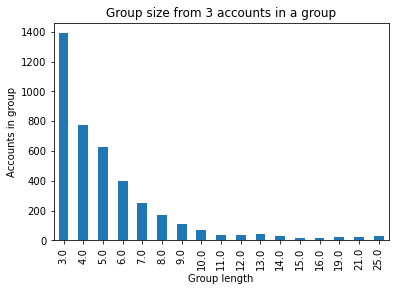
\includegraphics[width=0.2\textwidth]{group_size}\label{fig:f1}}
  \hfill
  \subfloat[Negative]{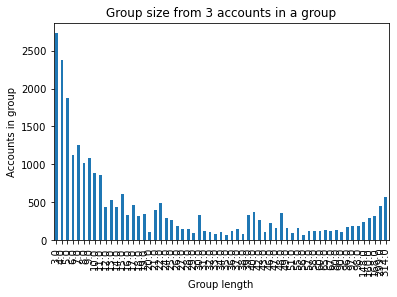
\includegraphics[width=0.2\textwidth]{group_size_negative}\label{fig:f2}}
  \caption{Groups}
\end{figure}


\begin{figure}[H]
  \centering
  \subfloat[Positive]{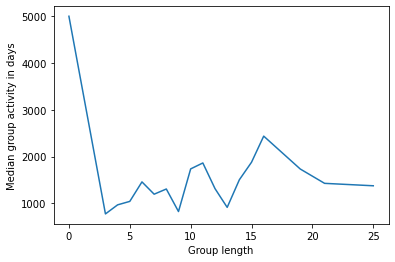
\includegraphics[width=0.2\textwidth]{group_activity}\label{fig:f1}}
  \hfill
  \subfloat[Negative]{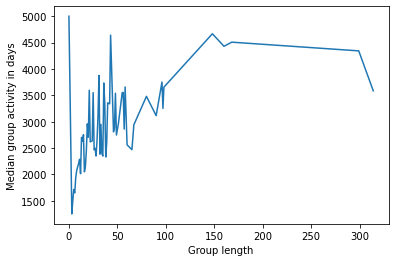
\includegraphics[width=0.2\textwidth]{group_activity_negative}\label{fig:f2}}
  \caption{Activity}
\end{figure}

\begin{figure}[H]
  \centering
  \subfloat[Positive]{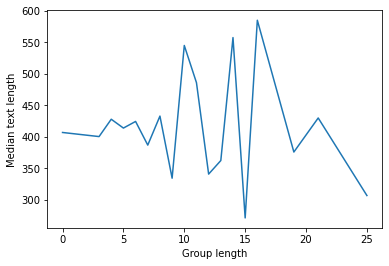
\includegraphics[width=0.2\textwidth]{len_review}\label{fig:f1}}
  \hfill
  \subfloat[Negative]{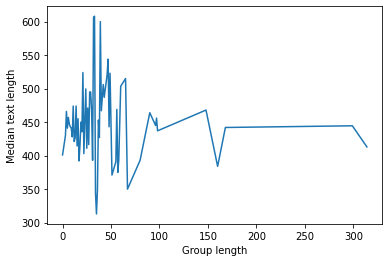
\includegraphics[width=0.2\textwidth]{len_review_negative}\label{fig:f2}}
  \caption{Length}
\end{figure}

\begin{figure}[H]
  \centering
  \subfloat[Positive]{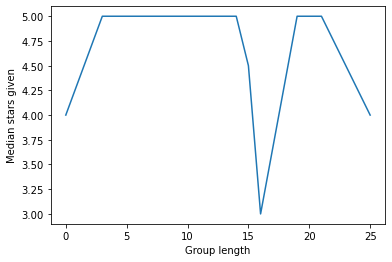
\includegraphics[width=0.2\textwidth]{stars_given}\label{fig:f1}}
  \hfill
  \subfloat[Negative]{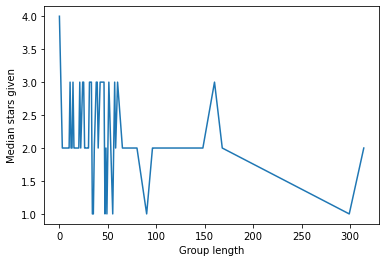
\includegraphics[width=0.2\textwidth]{stars_given_negative}\label{fig:f2}}
  \caption{Stars}
\end{figure}



% insert your bibliographic references into the bib.bib file
\bibliographystyle{plain}
\addcontentsline{toc}{section}{Bibliography}% Add to the TOC
\bibliography{bib}
\end{document}
